\chapterauthor{Andreas Lackner}

\chapter{Arbeitspaket Sensorik}
Die Analyse, Implementierung und Integration, sowie der Aufbau der ben\"otigten Schaltungen f\"ur die Sensorik des Experimentierplatzes, war Aufgabe von Herrn Lackner mit Unterst\"utzung von Herrn Brunner f\"ur Hardware-relevante Problemstellungen.

\section{\"Uberblick}
Um den Betrieb des Motorexperimentierplatzes zu erm\"oglichen und sinnvolle Anwendungen zu finden, m\"ussen eine Reihe von relevanten Kenngr\"o{\ss}en, durch den Einsatz von Sensorik, gemessen und diversen Modulen, bzw. den Benutzern des Experimentierplatzes zur Verf\"ugung gestellt werden. \\
Die zu erfassenden Daten, die in der Analysephase des Projekts festgelegt wurden, ergeben sich haupts\"achlich aus den bereits verbauten und uns so zug\"anglichen Sensoren. Gemessen werden folgende Werte:
\begin{itemize}
\item \textbf{Drehwinkel} \\
Aktueller Winkel der Motorwelle, relativ zu einem Festgelegten Nullpunkt.
\item \textbf{Drehgeschwindigkeit} \\
Umdrehungen der Welle pro Zeiteinheit.
\item \textbf{Motor-Temperatur} \\
Temperatur des Motors, da dieser sich im Betrieb erhitzt.
\item \textbf{Hall Pattern} \\
Stellt eine alternative M\"oglichkeit da, den Drehwinkel zu ermitteln. Das Pattern wird haupts\"achlich zur Kommutierung eingesetzt, da sich daraus sowohl der passende Zeitpunkt als auch das korrekte Motor-Pattern ableiten lassen.
\end{itemize}
Für die Ermittlung definierten Werte stehen auf den Experimentierstand drei \textbf{Hall-Sensoren}, ein \textbf{Inkrementalgeber} und ein \textbf{Temperatursensor} zur Verfügung, die alle im Aufbau fest verbaut sind. 

\section{Entwicklungsumgebung}
Wie auch die anderen Module, die direkt mit dem aufgebauten Motor interagieren, befindet sich die gesamte Software für die Sensorik auf dem Steuerungsmikrocontroller. Diese Aufgabe erfüllt momentan ein \textbf{XMC4800} von Infineon, aufgebaut auf einem Relax Kit V1. Da die Interaktion mit den Sensoren Hardware-nahe Programmierung erfordert, ist sämtlicher Code in C geschrieben. Als IDE für die Entwicklung dient DAVE 4 von Infineon.

\subsection{DAVE 4}
DAVE ist eine von Infineon bereitgestellte Entwicklungsumgebung für das Firmeneigene Controller Portfolio. Die Installationsdatei kann nach Registrierung bei Infineon direkt heruntergeladen werden. Während des Installationsprozesses werden ebenfalls automatisch die benötigten Treiber für den Debug-Chip auf dem Entwicklungsboard mit installiert. \\

\subsubsection{Projekt anlegen} 
DAVE bietet Standardm\"a{\ss}ig mehrere verschiedene Projekttypen an, die eine unterschiedliche Menge von bereits fertigem Code mit sich bringen. Bei einem \textbf{Empty Project} wird nur die HAL Bibliothek und die f\"ur den Controller ben\"otigten Startup Dateien bereitgestellt. Das \textbf{Simple Main} Projekt erstellt zus\"atzlich noch eine main.c Datei, mit einer leeren Main-Funktion. Entscheidet man sich für ein \textbf{Easy Start} Projekt, erh\"alt man Beispielcode der exemplarisch eine AD Wandlung vornimmt und einige Ausg\"ange setzt.

\begin{figure}[ht]
\centering
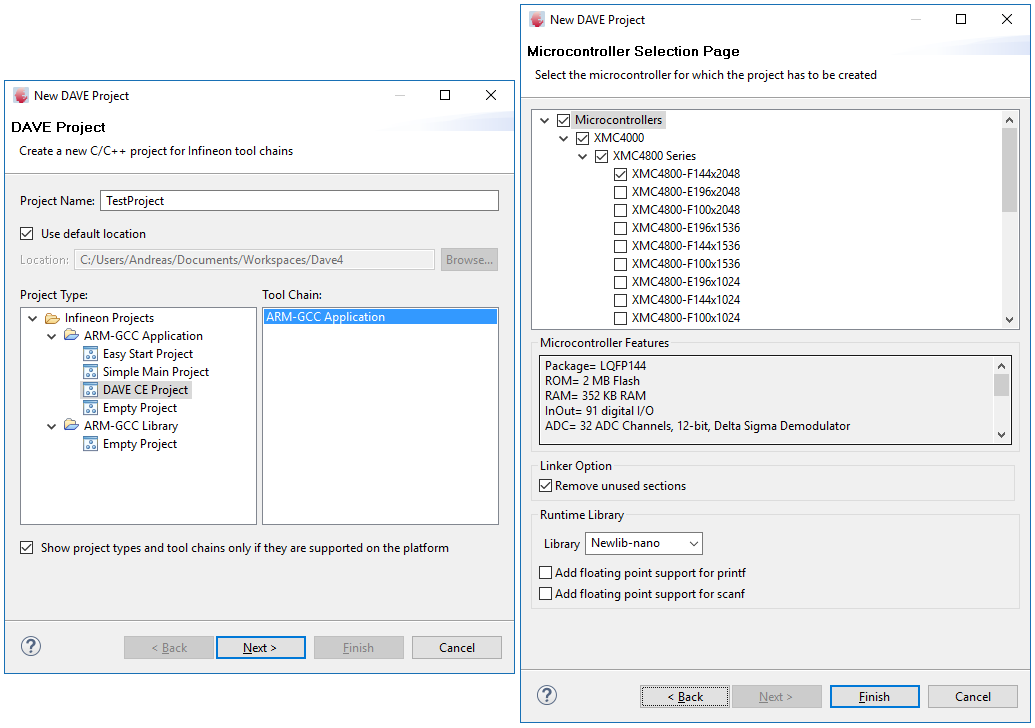
\includegraphics[width=\textwidth]{sensor/dave_project.PNG}
\caption{Projektdialog DAVE}
\label{img:dave_project}
\end{figure}

Einen Sonderfall bei den zur Auswahl stehenden Projektvorlagen stellen \textbf{DAVE CE} Projekte da. Diese Art von Projekt, ermöglicht die Verwendung von grafischen Oberflächen für die Konfiguration der Hardwareabstraktion. Dies umfasst unter anderem die Verbindung einzelner Komponenten untereinander oder mit den Pins des Mikrocontrollers, sowie grafische Konfigurationsformulare für die Komponenten selbst (z.B. ADC, CCU, POSIF, DIO usw.). \\ \\
Nach Wahl des Projektnamens und des gewünschten Projekttyps, muss auf der zweiten Seite des Dialogs der verwendete Mikrocontroller ausgewählt werden, um die korrekte Hardwarebibliothek bereitstellen zu können. Ein exemplarisches Beispiel für die Projekterstellung befindet sich in Abbildung \ref{img:dave_project}. 

\subsubsection{Projekt erstellen und herunterladen}
Um ein zu testendes Projekt auf den Controller herunterzuladen, muss es erst \textbf{kompiliert} werden. Gestartet wird der Buildprozess über den in Abbildung \ref{img:dave_build} markierten Button in der Menüleiste. 

\begin{figure}[ht]
\centering
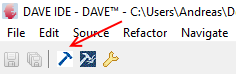
\includegraphics{sensor/dave_build.PNG}
\caption{Buildprozess starten}
\label{img:dave_build}
\end{figure}

\noindent
Im Anschluss an einen erfolgreichen Erstellungsprozess wird eine \textbf{Debug- bzw. Run-Konfiguration} angelegt. Diese umfasst alle für das Flashen benötigten Parameter wie Ort der zu ladenden Binärdatei sowieso GDB Konfigurationen.\\

\noindent
\fbox{\parbox{\linewidth}{Es ist wichtig, dass das Projekt vor dem Anlegen der Konfiguration einmal erstellt wird, da sonst wichtige Parameter nicht automatisch eingetragen werden.}} \\

\noindent
Das exemplarische Anlegen einer Debug-Konfiguration wird in Abbildung \ref{img:dave_debugConfig} gezeigt. Dafür wird im Fenster \textit{Debug Configurations} durch Doppelklick auf den eingesetzten Debug-Chip automatisch eine fertige Konfiguration angelegt.

\begin{figure}[ht]
\centering
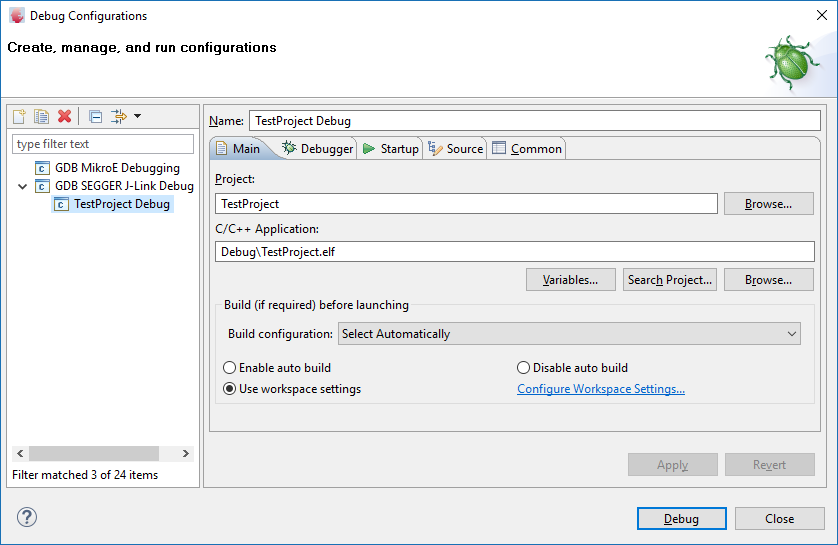
\includegraphics[width=0.8\textwidth]{sensor/dave_debugConfig.PNG}
\caption{Debug-Konfiguration erstellen}
\label{img:dave_debugConfig}
\end{figure}

\paragraph{Wichtiger Hinweis!} Es kann vorkommen, dass aus bisher unbekannten Gründen falsche GDB Startup-Skripte generiert werden, die beim Versuch das Projekt zu Debuggen, den sofortigen Abbruch des Vorgangs zur Folge haben. Es muss Sichergestellt werden dass in der Debug-Konfiguration, im Tab \textit{Startup}, unter dem Punkt \textit{Run/Restart Commands} keine Anweisungen eingetragen sind! \\

\noindent
Nach dem eine korrekte Konfiguration erstellt ist, kann das Programm über den Debug-Button in der Menüleiste auf den Controller geladen werden. DAVE wechselt im Anschluss automatisch in die Debug-Ansicht und unterbricht die Ausführung bei der ersten Anweisung in der Main-Funktion.

\subsection{POSIF}
\label{lbl:sensor_posif}
Das POSIF Modul der XMC Controller ist eigens auf den Betrieb von Motoranwendungen zugeschnitten. Dabei übernimmt es, in Kooperation mit einigen Caputure Compare Units, den kompletten Workflow vom einlesen verschiedener Sensoren für die Bestimmung der Kommutierungszeitpunkte bis hin zur Ansteuerung des Motors, bzw. dem setzen der Ausgänge um die Spulen anzusteuern. Ein allgemeiner Aufbau befindet sich in Abbildung \ref{img:posif_overview}.

\begin{figure}[ht]
\centering
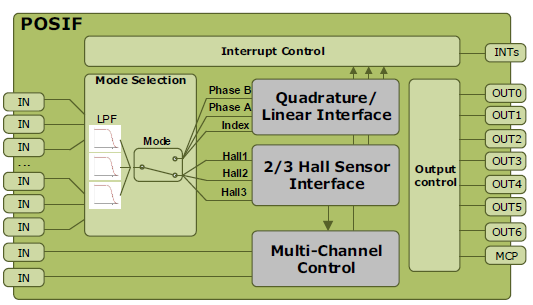
\includegraphics[width=0.8\textwidth]{sensor/posif_overview.PNG}
\caption{POSIF Übersicht}
\label{img:posif_overview}
\end{figure}

Im wesentlichen verfügt das POSIF Modul über zwei verschiedene Betriebsmodi zum einlesen des Zustands, die Optional mit dem Modul für die Motoransteuerung kombiniert werden können.

\begin{itemize}
\item \textbf{Hall Modus} \\
In diesem Betriebsmodus werden dem POSIF Modul die Signalpegel der Hall-Sensoren zugeführt. Wird eine Änderung detektiert, wird das gemessene Pattern, automatisch mit dem erwarteten verglichen und es wird entweder ein Interrupt für ein \textit{Correct-Hall-Event} oder ein \textit{Wrong-Hall-Event} ausgelöst. In der Interruptroutine muss im Code das Register für das aktuelle und erwartete Hall-Pattern aktualisiert werden, um den reibungslosen Betrieb zu ermöglichen.
\item \textbf{Quadrature Decoder Modus} \\
Dieser Modus verwendet als Informationsquelle einen Inkrementalgeber, der eine Indexleitung, sowie zwei Phasen A und B bereitstellt (alternativ kann auch ein Encoder mit nur \textit{Direction-} und \textit{Count-Leitung} verwendet werden). Unter Zuhilfenahme einer kompletten CCU lassen sich sowohl Umdrehungsgeschwindigkeit als auch Drehwinkel berechnen.
\end{itemize}

\section{Sensor Interface}
Sämtliche Funktionen die das Auslesen der definierten Sensorwerte ermöglichen sollen, sind in ein eigenes Softwaremodul gekapselt, dass die gewünschte Funktionalität über festgelegte Schnittstellen anbietet. \\

\begin{lstlisting}[frame=single, language=c, caption=Sensor Interface, label=lst:SensorInterface]
void Sensor_Init();

void Sensor_StartAll(void);

void Sensor_StopAll(void);

void Sensor_SetDirection(MotorDirection_t direction);

Std_ReturnType Sensor_RegisterHallCallback(HallCallbackType callback);

Std_ReturnType Sensor_GetCurrentHallPattern(HallPattern_t* pattern);

Std_ReturnType Sensor_GetVelocity(double* velocity);

Std_ReturnType Sensor_GetAngle(double* angle);

Std_ReturnType Sensor_GetTemperature(int* temperature);
\end{lstlisting}

\subsection{Modulstruktur}
Das angebotene Interface über die Sensor.h Datei, fungiert nur als Schnittstelle zu den Implementierungen der einzelnen Sensoren. Die Aufteilung in Submodule leitet sich dabei aus den verschiedenen Sensortypen her. \\
\dirtree{%
.1 Sensor.
.2 Sensor\_Types.h.
.2 Sensor\_Hall.h.
.2 Sensor\_QuadratureDecoder.h.
.2 Sensor\_Temperature.h.
}
\noindent \\
Alle Submodule bringen zum jetzigen Zeitpunkt ihre Abhängigkeiten\footnote{Mit Abhängigkeiten sind in erster Linie Konfigurationen der Hardwareelemente wie CCU, ADC oder POSIF gemeint.} schon mit, um den Integrationsaufwand in das fertige Projekt so gering wie möglich zu halten. Dies kann sich zu einem späteren Zeitpunkt noch ändern, wenn die POSIF Konfiguration für das einlesen der Hall-Sensoren mit der Motorsteuerung zusammengezogen wird, da beide Module auf die selbe Hardwarekomponente zugreifen.

\subsection{Anwendung}
Um Sensorwerte über das Softwaremodul einzulesen muss beim Startvorgang der Steuerung einmal die \textit{Sensor\_Init()} Funktion aufgerufen werden um alle eingesetzten Hardwarekomponenten zu initialisieren. Zu diesem Zeitpunkt sollte auch ein Callback für die Hall-Events registriert werden, um über eintretende Änderungen der Motorwelle informiert zu werden. Registrieren lässt sich eine Callback-Funktion über \textit{Sensor\_RegisterHallCallback(<func\_ptr>)}. \\
Vor dem Start muss dem Sensormodul ebenfalls die gewünschte Drehrichtung des Motors, über die Funktion \textit{Sensor\_SetDirection(<motor\_dir>)} mitgeteilt werden, um das korrekte Hall-Pattern ermitteln zu können. \\
Der Einlesevorgang für die Sensorwerte muss im Anschluss über die Funktion \textit{Sensor\_StartAll()} gestartet werden, und lässt sich über \textit{Sensor\_StopAll()} anhalten. \\

\noindent
Während des Regelbetriebs lassen sich die einzelnen Werte über die restliche API auslesen.

\begin{itemize}
\item \textbf{Sensor\_GetCurrentHallPattern(HallPattern\_t*)} Gibt das Muster zurück, dass sich auch den aktuelle Zustand der digitalen Hall-Sensoren ergibt. HallPatter\_t* beschreibt dabei einen Pointer auf die Hall-Pattern Struktur die durch den Funktionsaufruf mit Werten gefüllt wird.
\item \textbf{Sensor\_GetVelocity(double*)} Gibt die aktuelle Umdrehungsgeschwindigkeit der Motorwelle in Umdrehungen pro Sekunde zurück.
\item \textbf{Sensor\_GetAngle(double*)} Gibt den aktuellen Drehwinkel in Grad, relativ zu einem festgelegten Nullpunkt zurück.
\item \textbf{Sensor\_GetTemperature(int*)} Gibt die aktuelle Temperatur in Grad Celsius im Motor zurück.
\end{itemize}

\section{Hall Sensoren}
Ein Hall-Sensor misst magnetische Flussdichte, durch die Ausnutzung des Hall-Effekts. In unserem Versuchsaufbau sind drei dieser Sensoren, jeweils im Winkel um 120$^\circ$ versetzt, im Motor verbaut (Abbildung \ref{img:hall_sample}). Es handelt sich dabei um digitale Sensoren, was bedeutet dass der gemessene Sensor-Wert entweder logisch 1 oder 0 ist.

\begin{figure}[ht]
\centering
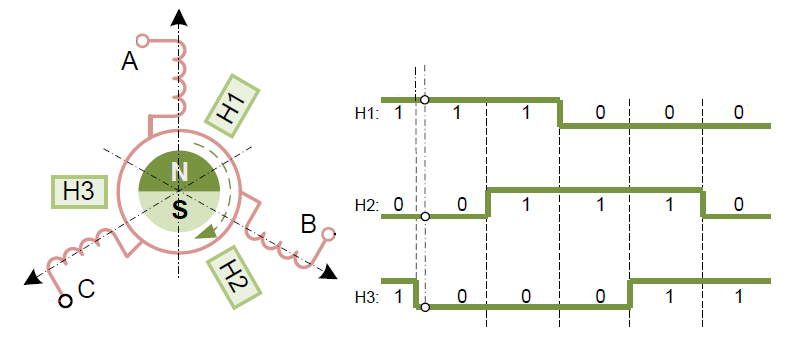
\includegraphics[width=0.8\textwidth]{sensor/hall_sample.PNG}
\caption{Hall Sensoren und Pattern}
\label{img:hall_sample}
\end{figure}

Der Wert ändert sich dabei in Abhängigkeit davon, ob sich grade ein magnetischer Nord- bzw. Südpol über den Sensor befindet. Alle drei Sensorzustände zusammen genommen ergeben ein \textbf{Hall-Pattern}, was im rechten Teil von Abbildung \ref{img:hall_sample} noch einmal verdeutlicht wird. Das Hall-Pattern ist relevant für zwei Dinge. Zum einen kann Anhand des gemessenen und des erwarteten Pattern festgestellt werden, ob beim Drehvorgang Fehler aufgetreten sind (z.B. ob der Motor sich in die falsche Richtung dreht) und zum anderen lässt sich aus dem Zeitpunkt des Auftretens einer Änderung des Musters, eine passende Gelegenheit für die Kommutierung ableiten. Bei gewissen Regelstrategien lässt sich außerdem aus dem Hall-Pattern ein Motor-Pattern ableiten, welches an die Spulen angelegt wird um eine Drehung des Motors zu erzeugen.

\subsection{Einlesen der Hall-Sensoren}
Die für uns effizienteste Möglichkeit das Hall-Pattern einzulesen und seine Korrektheit zu prüfen ist die Verwendung des in Kapitel \ref{lbl:sensor_posif} beschriebenen POSIF Moduls (POSition InterFace), dass die Verwendeten XMC Mikrocontroller mitbringen.\\

\noindent
In der verwendeten Konfiguration benötigt der Hall-Modus zwei CCU Slices. Wird vom POSIF Modul die Änderung der Eingänge detektiert, startet es das erste CCU Slice als Debounce Timer, um auszuschließen dass die Statusänderung ihren Ursprung in einem Fehlerhaften Signal hat. Anschließend erfolgt der Vergleich, mit dem im Register abgelegten erwarteten Pattern, was entweder die Generierung eines Correct-Hall-Events oder Wrong-Hall-Events zur Folge hat. Im Fall eines CHE, löst die Software das registrierte Hall-Callback aus, um die Motorsteuerung über das eingetretene Ereignis zu benachrichtigen. Ebenfalls wird im Anschluss daran, das Register für das nächste erwartete Hall-Pattern aktualisiert. Das zweite CCU Slice kann verwendet werden, um auf Basis der auftretenden Hall-Events die aktuelle Umdrehungsgeschwindigkeit bzw. den Winkel der Motorwelle zu berechnen.

\subsection{Ermittlung der Hall-Pattern}
Der reibungslose Betrieb des Hall Moduls im Sensor Interface setzt voraus, dass das Register des POSIF Moduls immer mit dem korrekten, erwarteten Hall-Pattern befüllt wird. Dieses Muster unterscheidet sich je nach verwendetem Motor, und musste in unserem Fall extra ausgemessen werden. Dazu habe ich die Hall-Sensoren mit Spannung versorgt und an jede der drei Leitungen ein Oszilloskop gehängt. Durch händisches Drehen des Motors wird die gewünschte Abfolge sichtbar (abgebildet in Abbildung \ref{img:hall_pattern}).

\begin{figure}[ht]
\centering
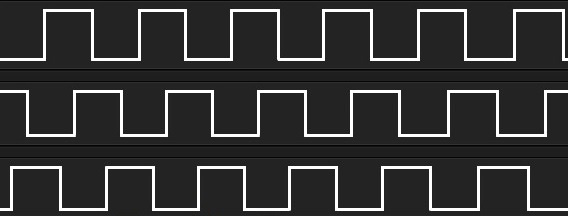
\includegraphics[width=0.8\textwidth]{sensor/hall_pattern.jpg}
\caption{Eingelesenes Hall-Pattern}
\label{img:hall_pattern}
\end{figure}

Auf Basis dieser Messung lässt sich durch festlegen eines beliebigen Startpunkts das Hall-Pattern für die gewählte Drehrichtung ableiten. Ab dem gewählten Startpunkt führt jede Änderung des Zustands zu einem neuen Pattern. Die Analyse hat für unseren Motor hat 6 verschiedene Pattern ergeben, die sich pro Umdrehung 7-Mal wiederholen. Dies ergibt eine Gesamtzahl von 42 Hall-Events pro Umdrehung. Das gleiche Verfahren wurde zu Überprüfungszwecken auch mit der zweiten Drehrichtung durchgeführt, um Fehler zu vermeiden. 

\begin{figure}[ht]
\centering
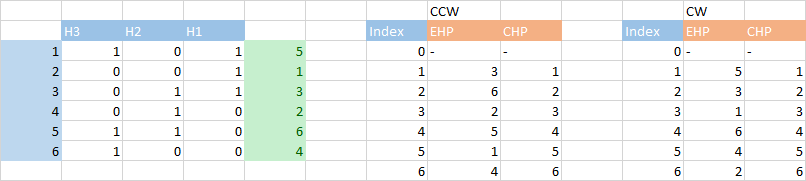
\includegraphics[width=\textwidth]{sensor/hall_pattern_lookup.PNG}
\caption{Hall-Pattern Lookup-Tables}
\label{img:hall_pattern_lookup}
\end{figure}

Um einen effizienten Wechsel der Pattern zu garantieren, wird eine Lookup-Table eingesetzt, die das aktive Hall-Pattern als Index nutzt, um das nächste erwartete Pattern zu finden. Die genaue Struktur der Tabelle ist in Abbildung \ref{img:hall_pattern_lookup} aufgeschlüsselt.

\section{Inkrementalgeber}
Für die Berechnung der Umdrehungsgeschwindigkeit und des aktuellen Winkels steht ein Inkrementalgeber zur Verfügung, der über eine Indexleitung Z und zwei Phasen A und B verfügt. Der Sensor selbst ist mit der Motorwelle gekoppelt und verändert seine Leitungspegel mit den Drehbewegungen der Welle. \\

Die Umdrehungsgeschwindigkeit lässt sich über die Indexleitung errechnet, die pro vollständiger Umdrehung der Welle an einem definierten Punkt für kurze Zeit einen High-Pegel annimmt. Der Winkel sowie die Drehrichtung lassen sich über die Phasen A und B ermitteln. Wie in Abbildung \ref{img:quadrature_overview} gezeigt, wechseln sowohl A als auch B immer zwischen einem High- und Low-Zustand. Da nicht beide Phasen gleichzeitig den Pegelwechsel vollziehen, sondern je nach Drehrichtung eine Phase vor der anderen, lässt sich daraus die Drehrichtung ableiten. Den aktuellen Winkel erhält man durch Mitzählen, da pro Umdrehung immer die gleiche definierte Anzahl an Flankenwechsel durchgeführt werden. Der absolute Winkel, relativ zum Nullpunkt den die Indexleitung vorgibt, erhält man durch die Formel \ref{eq:angle}.

\begin{equation}
\label{eq:angle}
angle = (edge_count / total_edges) * 360
\end{equation}

\begin{figure}[ht]
\centering
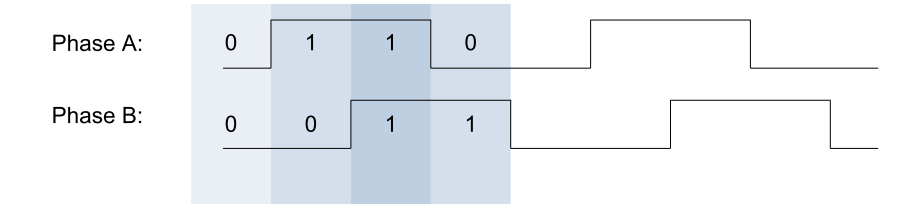
\includegraphics[width=\textwidth]{sensor/quadrature_overview.PNG}
\caption{Inkrementalgeber Phasen}
\label{img:quadrature_overview}
\end{figure}

\subsection{Implementierung}
Für das Einlesen und die Verarbeitung der Leitungssignale des Inkrementalgebers wird das im Kapitel \ref{lbl:sensor_posif} beschriebene POSIF Modul im Quadrature Decoder Modus herangezogen. Durch zuführen der Phasen und der Indexleitung errechnet die verwendete POSIF Instanz sechs verschiedene Ausgänge. 

\begin{itemize}
\item Auftreten des Indexsignals
\item Fertige Umdrehung
\item Drehrichtung
\item Quadrature Clock
\item Period Clock
\item Synchronisierter Start
\end{itemize}
 
In Kombination mit passend konfigurierten CCU Slices lassen sich Anhand der internen Ausgänge des POSIF Moduls die angestrebten Kenngrößen ermitteln.


\section{Temperatursensor}
Der eingesetzte Sensor für die Ermittlung der Temperatur im Motor verwendet einen NTC-Widerstand (Negative Temperature Coefficient) für die Temperaturermittlung. Bei dieser Bauform, sinkt der Widerstand des Sensors bei steigender Temperatur. Die bei uns verbaute Variante deckt einen Temperaturbereich von -40$^\circ$ bis 110$^\circ$ Celsius ab und verfügt über einen Basiswiederstand von 10kOhm bei einer Temperatur von 25$^\circ$ Celsius.

\subsection{Einlesen des Temperaturwerts}
Für die Ermittlung des aktuellen Temperaturwerts ist es notwendig den Widerstandswert des Sensors einzulesen und zu digitalisieren. Da sich der Widerstand nicht direkt messen lässt wird ein Spannungsteiler eingesetzt, dessen Spannung am Messpunkt sich proportional zum Widerstand verhält. Diese Messspannung kann am Controller über einen AD-Wandler eingelesen werden.

\begin{figure}[ht]
\centering
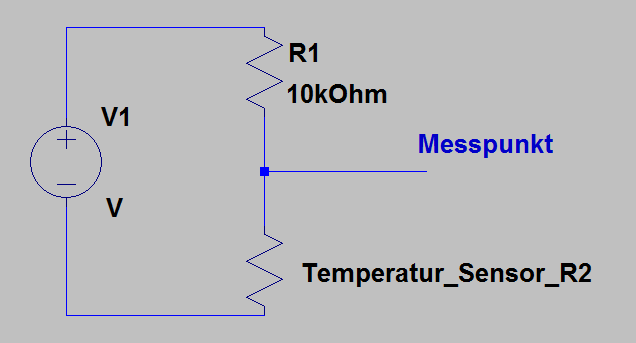
\includegraphics[width=0.65\textwidth]{sensor/temperature_circuit.PNG}
\caption{Spannungsteiler zum einlesen des NTC-Widerstands}
\label{img:temperature_circuit}
\end{figure}

Der genaue Schaltungsaufbau lässt sich aus Abbildung \ref{img:temperature_circuit} entnehmen. Als fixer Widerstand werden 10kOhm verwendet. Dieser Wert spielt später bei der Errechnung des Widerstands des Temperatursensors T1 eine Rolle. Nach anlegen einer Versorgungsspannung lässt sich die variable Spannung am Messpunkt abgreifen. \\
\label{lbl:temp_equation}
Um aus der gemessenen Spannung den Widerstand zu errechnen, muss zunächst von der Formel für $U_{2}$ des Spannungsteiler ausgegangen werden.

\begin{equation}
U_{2} = \frac{U_{ges}}{R_{1} + R_{2}} * R_{2}
\end{equation}

Bekannt sind in dieser Formel die Werte für $U_{ges}$, die gemessene Spannung $U_{2}$ und der Widerstand $R_{1}$. Durch Äquivalenzumformung lässt sich die Formel auf den gewünschten Wert $R_{2}$ umstellen.

\begin{equation}
R_{2} = \frac{U_{2} * R_{1}}{U_{ges} - U_{2}}
\end{equation}

Ist der Widerstand bekannt, lässt sich aus dem Datenblatt des Sensors die dazu passende Temperatur ermitteln.

\subsubsection{Analog Digital Wandlung}
Die ADC Einheit des XMC Controllers verfügt über vier unabhängige Konvertierungsgruppen mit bis zu 8 analogen Eingängen und einer maximalen Auflösung von 12 Bit. Standard Referenzspannung sind dabei 3.3 Volt.

\begin{figure}[ht]
\centering
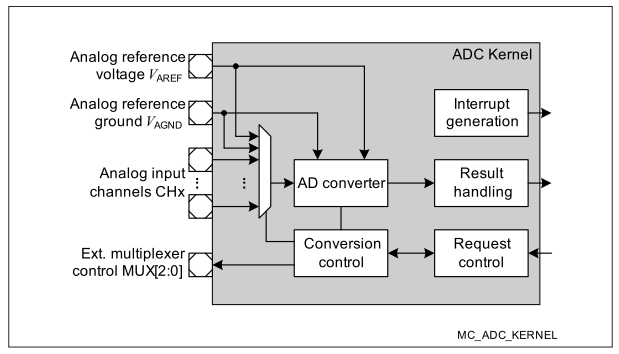
\includegraphics[width=0.9\textwidth]{sensor/xmc_adc.PNG}
\caption{ADC Einheit der XMC Controller}
\label{img:xmc_adc}
\end{figure}

Für die Wandlung stehen drei verschiedene Modi zur Verfügung: 
\begin{itemize}
\item \textbf{Fixed Channel Conversion} \\
Ein einzelner festgelegter Kanal wird konvertiert.
\item \textbf{Auto Scan Conversion} \\
Alle verfügbare Kanäle werden in einer konfigurierbaren Sequenz automatisch und linear gewandelt.
\item \textbf{Channel Sequence Conversion} \\
Konvertierung von 8 willkürlich gewählten Kanälen.
\end{itemize}

Jeder dieser Modi kann entweder einmalig auf explizite Anfrage, oder kontinuierlich eine Konvertierung durchführen. Als Quelle der Anfragen stehen ebenfalls mehrere Einheiten zur Verfügung (zwei Group-Request-Sources und eine Background-Request-Source). Da von mehreren Quellen Anfragen gleichzeitig eintreffen können, wird die Reihenfolge der Abarbeitung von einem Arbiter festgelegt. Der genaue Aufbau einer einzelnen ADC Einheit lässt sich der Abbildung \ref{img:xmc_adc} entnehmen. \\

In unserem konkreten Beispiel wird eine Fixed-Channel-Konvertierung durchgeführt, da nur ein einzelner Kanal eingelesen werden muss. Das absetzen der Anfrage wird dabei von der Background-Request-Source übernommen. Da die Konvertierung einige Mikrosekunden Zeit benötigt, wird nach Abschluss des Vorgangs ein Interrupt ausgelöst.

\subsubsection{Implementierung}
Die Ermittlung des aktuellen Temperaturwerts wird nur auf Anfrage durch die Sensor API ausgeführt. Die im Codesnippet \ref{lst:temp_calculation} aufgeführte Funktion, startet die Konvertierung und wartet durch Busy-Waiting auf deren Abschluss. Zu dem gemessenen Spannungswert wird wie bei \ref{lbl:temp_equation} aufgeführt, der zugehörige Widerstandswert berechnet. Der passenden Temperaturwert wird durch die Suche in einer sortierten Tabelle ermittelt.

\begin{lstlisting}[frame=single, language=c, caption=Temperaturberechnung, label=lst:temp_calculation]
int Sensor_Temperature_Calculate(Sensor_TemperatureType sensor)
{
	int i = 0;
	double adcVoltage = 0;
	double res = 0;

	/* Start measurement */
	MeasurementRunning = 1;
	Sensor_Temperature_ADC_StartConversion();

	/* Wait for measurement to finish*/
	while(MeasurementRunning == 1);

	/* Calculate temperature */
	adcVoltage = ConvertToVoltage(SensorVoltages[sensor]);
	res = (adcVoltage * R1) / (SENSOR_REF_VOLTAGE - adcVoltage);

	while(TemperatureLookupTable[i++].resistence > res && 
			i < NTC_LOOKUP_ENTRIES);

	return TemperatureLookupTable[i].temperature;
}
\end{lstlisting}

\section{Ausblick}
Momentan befindet sich der Code für das Einlesen der Sensorwerte vom Inkrementalgeber noch in Entwicklung. Bei der aktuellen Bearbeitungslage ist eine vollständige Fertigstellung nicht absehbar. \\
Basierend auf der Ideensammlung aus der Analysephase wäre eine mögliche Erweiterung dieses Arbeitspakets die Portierung auf andere Controller. Durch das mögliche Fehlend des POSIF Moduls auf anderen Plattformen wird dadurch eine Neuimplementierung für das Einlesen der Hall-Sensoren sowie des Inkrementalgebers notwendig. \\ \\
Eine weitere Aufgabe wäre die Kommutierung nicht von den Hall-Events abhängig zu machen, sondern als Basis den Inkrementalgeber zu verwenden. Dies ermöglicht die Verwendung neuer Kommutierungsstrategien und stellt mit Sicherheit eine interessante Erweiterung des Funktionsumfangs da.